\subsection{Ejercicio 1}
	Este primer ejercicio del trabajo práctico consistió en crear una tabla de descriptores globales (\code{GDT}) básica, para luego pasar el 
procesador a modo protegido y escribir en la memoria de vídeo el marco sobre el cual estará el resto del trabajo.

 	El código escrito se dividió en definir la \code{GDT} en el archivo \code{gdt.c} y el resto en el archivo principal \code{kernel.asm}.

\subsubsection{\code{gdt.c}}
	El archivo consiste en un array de estructuras \code{gdt\_entry} definidas en \code{gdt.h}. La estructura describe un descriptor global 
que mide 8 \keyword{bytes}.
	Se compone de bits reservados para el tamaño (\code{limit}), la dirección base del segmento a describir (\code{base}), y diversos atributos 
que serán explicados a continuación junto con los segmentos que definimos:

\noindent La \code{gdt} define cuatro descriptores en el siguiente orden:
\begin{itemize}
	\item Descriptor nulo
	\item Descriptor para el segmento de código
	\item Descriptor para el segmento de datos
	\item Descriptor para el segmento que apunta a la memoria de video.
\end{itemize}

\begin{center}
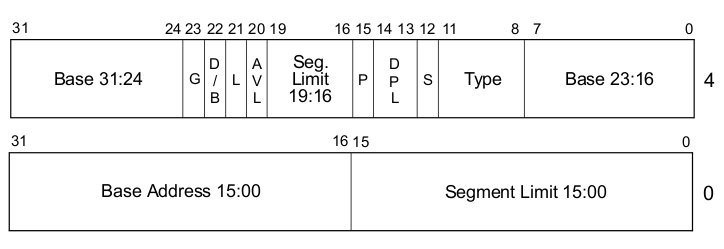
\includegraphics[scale=0.3]{gdt_descriptor.png}
\end{center}

\noindent \textbf{Campos de cada descriptor}:
\begin{itemize}
	\item\code{Limit}: Indica el tamaño de cada segmento definido. En las entradas de código y datos estos \keyword{bits} están seteados a su máximo valor, 
que junto con la base y el \keyword{bit} de \keyword{granularity} van a formar dos segmentos de 4gb cada uno. En el segmento de video el tamaño es de 4kb, 
o sea, una página.
	\item\code{Base}: Indica en que posición de memoria empiezan los segmentos. Tanto el segmento de código como el de datos tienen como base al 
\code{0x0000}, para poder lograr el tamaño final de 4gb. El segmento de vídeo empieza en \code{0x0B8000} según la especificación dada.
	\item\code{Type}: Este campo de 4 \keyword{bits}, indica si el segmento es de código o de datos y los permisos de lectura, escritura y ejecución 
entre otras cosas. Se decidió que el segmento de código lleve el valor \code{0xA} (según el manual de Intel, esto es segmento de código de lectura/escritura), 
el segmento de datos \code{0x2} (segmento de datos de lectura/escritura) y el segmento de video también \code{0x2}.
	\item\code{Bit S}: Indica si el segmento es de código/datos o de sistema. Para todos los segmentos se indica que es un segmento de código/datos.
	\item\code{Bit DPL}: Indica el nivel de privilegio que tiene el segmento. Todos los segmentos tienen privilegio a nivel \keyword{Kernel} (el máximo posible).
	\item\code{Bit P}: Indica si el segmento está presente. Para todos los segmentos, se indica que esta presente, sino al tratar de accederlo se 
produciría una excepción.
	\item\code{Bit AVL}: Irrelevante, seteado a 0.
	\item\code{Bit L}: Este \keyword{bit} indica si el segmento contiene código de 64 \keyword{bits}. Seteado a 0 para indicar que este no es el caso.
	\item\code{Bit D/B}: El \keyword{bit} funciona de manera diferente según se trate de un segmento de código, datos expand-down, o de stack. 
Lo único relevante en este punto es que en el segmento de código está seteado en 1 para que interprete direcciones de 32 \keyword{bits} y operandos de 32 u 8 \keyword{bits}, como es necesario en modo protegido.
	\item\code{Bit G}: Este \keyword{bit} (\code{granularity}) indica si el campo \code{limit} del segmento se interpreta como unidad de \keyword{bytes} (dando como máximo 1MB de tamaño de segmento) o como unidades de 4kb (dando el máximo de 4gb buscado). Para todos los segmentos, este \keyword{bit} esta seteado.
\end{itemize}

\subsubsection{\code{kernel.asm}}
	Luego de habilitar la A20 y detener las interrupciones, se carga el registro \code{GDTR} que apunta a la tabla de descriptores que fue explicada 
anteriormente. Para ello se utilizó la instrucción:

\vspace{2mm}
	\code{lgdt [GDT\_DESC]}
\vspace{2mm}

	A continuación se setea el \keyword{bit} 0 del registro de control \code{cr0}, poniendo el procesador en modo protegido, y se realiza un \code{jump far} 
al comienzo del código en modo protegido:

\begin{verbatim}
	mov eax, cr0
	or eax, 1
	mov cr0, eax
	jmp 0x08:modo_protegido
\end{verbatim}

\vspace{2mm}

	El \code{0x08} le indica al registro de segmento \code{CS} que apunte a esa dirección desde la dirección que apunta el \code{GDTR}. Que es donde 
está el descriptor de segmento de código que definimos antes. Luego se acomodan los demás registros de segmento al segmento de datos y se empieza con 
el código para escribir en pantalla.

	Para escribir en la pantalla se va a usar la instrucción \code{stosw}. La instrucción escribe un \keyword{word} guardado en \code{ax} en la 
dirección apuntada por \code{es:edi}. Entonces se carga el inicio del segmento de vídeo en el registro \code{es}, después se limpia la pantalla 
escribiendo \code{0x0000} en \code{ax} e incrementando el \keyword{offset} de \code{edi}. El registro \code{ecx} se utiliza para manejar el \keyword{loop}.

\begin{verbatim}
	mov ax, 0x18
	mov es, ax
	xor edi,edi
	mov ecx, (25 * 80)
	mov ax, 0x0000
	limpiarPantalla:
		stosw	
		loop limpiarPantalla
\end{verbatim}

	Posteriormente se realizan las rutinas simples para dibujar el marco de una manera similar a la recientemente mostrada.

